\documentclass[a4paper,landscape,twocolumn]{article}
\usepackage[utf8]{inputenc}
\usepackage[T1]{fontenc}
\usepackage[ngerman,english]{babel}
\usepackage{amsmath}
\usepackage{amssymb}
\usepackage{amsthm}
\usepackage{csquotes}
\usepackage{fancyhdr}
\usepackage[margin=1in]{geometry}
\usepackage[makeindex]{imakeidx}  % before hyperref
\usepackage[pdfborder={0 0 0}]{hyperref}
\usepackage{marvosym}
\usepackage{mathtools}
\usepackage{mdframed}
\usepackage{stmaryrd}
\usepackage[normalem]{ulem}
\usepackage{wasysym}

\parskip5pt
\parindent0pt

\theoremstyle{definition}

\newtheorem{theorem}{Theorem}
\newtheorem{defi}{Definition}
\newtheorem{rem}{Remark}
\newtheorem{ex}{Example}
\newtheorem{cor}{Corollary}
\newtheorem{lemma}{Lemma}

\newcommand\okay{\qquad\checkmark}
\newcommand\set[1]{\left\{#1\right\}}
\newcommand\setdef[2]{\left\{#1\,|\,#2\right\}}
\newcommand\abs[1]{\left|#1\right|}
\newcommand\seq[1]{{\left(#1\right)}_{n \in \mathbb N}}
\newcommand\card[1]{\left|\,#1\,\right|}
\newcommand\meta[3]{\hrule{} This #1 took place on #2 with lecturer #3.\par}
\newcommand\done{\hspace{10pt}\checkmark}
\newcommand\norm[1]{\left\|#1\right\|}

\pagestyle{fancy}
\fancyhf{}
\chead{\Large{\textsc{Mathematical Analysis II -- Lecture Notes}}}
\lfoot{\makebox[\columnwidth]{\thepage}}
\rfoot{\makebox[\columnwidth]{\number\numexpr\value{page}+1}\stepcounter{page}}
\setlength{\headheight}{18pt}

\makeindex[name={German},title={German keywords}]
\makeindex[name={English},title={English keywords}]
\twocolumn

\title{
  Mathematical analysis 2 -- Lecture notes \\
  \small{course by Wolfgang Ring}
}
\author{Lukas Prokop}
\date{March to July 2016}

\begin{document}
\maketitle
\tableofcontents

\clearpage
\meta{lecture}{1st of March 2016}{Wolfgang Ring}

Course organization:
\begin{itemize}
  \item Tuesday, 1 hours 30 minutes, beginning at 8:15
  \item Thursday, 45 minutes, beginning at 8:15
  \item Friday, 1 hours 30 minutes, beginning at 8:15
\end{itemize}

Literature:
\begin{itemize}
  \item Königsberger, Analysis 1
\end{itemize}

\clearpage
\section{Exponential function (cont.)}
%
Let $(z_n)_{n \in \mathbb N}$ be a complex series with $\lim_{n\to\infty} z_n = z$
and $\lim_{n\to\infty} (1 + \frac{z_n}{n})^n = \sum_{k=0}^\infty \frac{z^k}{k!}$.
For every complex number $z \in \mathbb C$ this series converges on entire $\mathbb C$.

\[ \exp(z) = \lim_{n\to\infty} \left(1 + \frac{z}n\right)^n = \sum_{k=0}^\infty \frac{z^k}{k!} \]
\[ \exp(z + w) = \exp(z) \cdot \exp(w) \]
\[ \lim_{z\to0} \frac{\exp(z) - 1}{z} = 1 \]
\[ \exp(1) = e \in \mathbb R \]
\[ z = \frac mn \in \mathbb Q \land n \neq 0 \Rightarrow \exp\left(\frac mn\right) = e^{\frac mn} \]

So we also denote
\[ \exp(z) = e^z \qquad \text{for } z \in \mathbb C \]
It holds that
\[ \exp(z) \neq 0 \qquad \forall z \in \mathbb C \]

$\exp(x)$ for $x \in \mathbb R$
\[ e^x > 0 \qquad \forall x \in \mathbb R \]

\[ (e^x)' = e^x \]
It follows immediately that the exponential function is strictly monotonically increasing in $\mathbb R$.
\[ (e^x)'' = (e^x)' = e^x > 0 \]
It follows that the exponential function is convex. But as usual,
\[ e^0 = 1 \]

\begin{figure}[!h]
  \begin{center}
    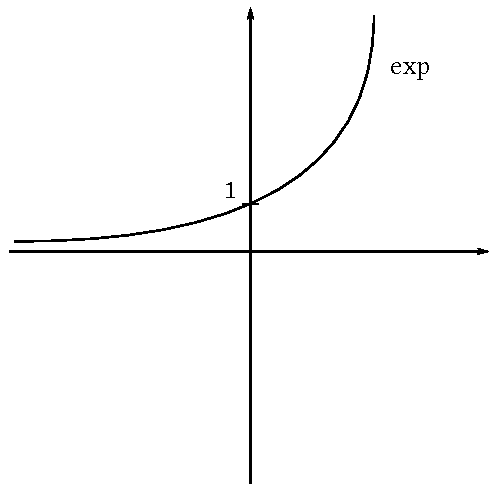
\includegraphics{img/exp-graph.pdf}
    \caption{Graph of the exponential function}
  \end{center}
\end{figure}

Let $n \in \mathbb N$
\[ \lim_{x\to+\infty} \frac{e^x}{x^n} = \infty \]
\[ \lim_{x\to-\infty} e^x \cdot x^n = 0 \]

\section{The natural logarithm}
%
\[ \exp: \mathbb R \to (0,\infty) \]
is injective, because $x_1 < x_2 \Rightarrow e^{x_1} < e^{x_2}$

\begin{lemma}
  $\exp: \mathbb R \to (0,\infty)$
  is surjective.
\end{lemma}
\begin{proof}
  We need to show that the equation $e^x = y$ has some solution for every $y > 0$.
  We will use the Intermediate Value Theorem, we discussed in the previous course \enquote{Analysis 1}.

  \begin{description}
    \item[Case 1]
      First of all, let $y \in [1,\infty)$. Then it holds that
      \[ e^0 = 1 \leq y \quad\text{and}\quad e^y = 1 + y + \underbrace{\frac{y^2}{2} + \frac{y^3}{3!} + \frac{y^4}{4!} + \ldots}_{\geq 0} \]
      \[ \geq 1 + y > y \]
      Therefore $e^0 \leq y < e^y$.
      Hence $\exp$ is continuous and the Intermediate Value Theorem applies:
      \[ \exists \xi \in [0,y]: \quad e^\xi = y \]
    \item[Case 2]
      Let $y \in (0,1)$. Then it holds that $w = \frac1{y} > 1$.
      The same as in Case~1 applies:
      \[ \exists \xi \in [0,w]: \quad e^\xi = w = \frac1{y} \]
      \[ \Rightarrow e^{-\xi} = \frac{1}{e^\xi} = y \]
  \end{description}

  So it holds that $\exp: \mathbb R \to (0,\infty)$ is bijective.
\end{proof}

\index[English]{Natural logarithm}
\index[German]{\foreignlanguage{ngerman}{Natürlicher Logarithmus}}
\begin{defi}
  We call the inverse function \emph{natural logarithm}\footnote{In non-German literature $\ln(y)$ is almost exclusively written with the more general $\log(y)$.}.
  \[ \exp^{-1}: (0,\infty) \to \mathbb R \]
  \[ \exp^{-1} = \ln(y) = \log(y) \]

  Properties:
  \begin{itemize}
    \item It holds $\forall x \in \mathbb R: \ln(e^x) = x$ and $\forall y \in (0,\infty): e^{\ln(y)} = y$.
    \item $\ln: (0,\infty) \to \mathbb R$ is strictly monotonically increasing
      \begin{proof}
        Let $0 < y_1 < y_2$. Assume $\ln(y_1) \geq \ln(y_2) \xRightarrow{\text{monotonicity}} e^{\ln(y_1)} \geq e^{\ln(y_2)} \Rightarrow y_1 \geq y_2$. Contradiction!
      \end{proof}
  \end{itemize}
\end{defi}

\subsection{Functional equations of logarithm}
%
\begin{itemize}
  \item
    For all $x,y > 0$ it holds that
    \[ \ln(x \cdot y) = \ln(x) + \ln(y) \]
  \item Limes:
    \[ \lim_{x \to 1} \frac{\ln(x)}{x - 1} = 1 \]
\end{itemize}
\begin{proof}
  \begin{itemize}
    \item
      \[ x \cdot y = e^{\ln(x \cdot y)} \]
      \[ e^{\ln(x)} \cdot e^{\ln(y)} = e^{\ln(x) + \ln(y)} \]
      Injectivity of $\exp$:
      \[ \ln(x \cdot y) = \ln(x) + \ln(y) \]
    \item
      Let $(x_n)_{n\in\mathbb N}$ with $x_n > 0$ be an arbitrary
      sequence with $\lim_{n\to\infty} x_n = 0$.
      Let $w_n = 1 + x_n$. Then it holds that
      $\lim_{n\to\infty} w_n = 1$ and $y_n = \ln(1 + x_n) = \ln(w_n)$.
      \[ \lim_{n\to\infty} y_n = \ln(1) = 0 \]
      \[ \lim_{n\to\infty} \frac{\ln(w_n)}{w_n - 1} = \lim_{n\to\infty} \frac{y_n}{e^{y_n} - 1} = \frac11 = 1 \]
      where
      \[ e^0 = 1 \Rightarrow \ln(1) = 0 \]
  \end{itemize}
\end{proof}

\begin{theorem}[Logarithmic growth]
  $\forall n \in \mathbb N_+$ it holds that $\lim_{n\to\infty} \frac{\ln(x)}{\sqrt[n]{x}} = 0$
\end{theorem}
\begin{proof}
  Let $x \in (0,\infty)$ with $x = e^{n\cdot\xi}$. That is,
  \[ \xi = \frac{\ln(x)}{n} \]
  \[ x \to \infty \Leftrightarrow \xi \to \infty \]
  \[
    \lim_{x\to\infty} \frac{\ln(x)}{\sqrt[n]{x}}
    = \lim_{\xi\to\infty} \frac{n \cdot \xi}{\sqrt[n]{e^{n \cdot \xi}}}
    = \lim_{\xi\to\infty} \frac{n \cdot \xi}{e^\xi} = 0
  \]
  because $n \cdot \xi < \xi^2$ for $\xi > n$ and $\lim_{\xi\to\infty} \frac{\xi^2}{e^\xi} = 0$.
\end{proof}

\begin{theorem}
  The logarithm function is differentiable in $(0,\infty)$ and it holds that $(\ln(x))' = \frac1x \quad \forall x > 0$.
\end{theorem}
\begin{figure}[!h]
  \begin{center}
    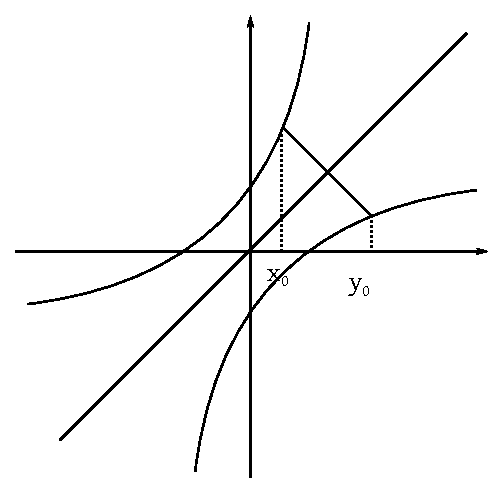
\includegraphics{img/geometric-exp-proof.pdf}
    \caption{A geometric proof of differentiability}
    \label{img:geo-diff}
  \end{center}
\end{figure}
\begin{proof}
  \begin{description}
    \item[First approach]
      Let $x > 0$, $x_n \to x$ with $x_n \neq x$, $x_n > 0$.
      Let $\xi_n = \ln(x_n)$ and $\xi = \ln(x) \Rightarrow \xi_n \neq \xi$.
      \[ e^{\xi_n} = x_n \qquad e^\xi = x \qquad \xi_n \to \xi \]
      Then it holds that
      \[ \lim_{n\to\infty} \frac{\ln(x_n) - \ln(x)}{x_n - x} = \lim_{n\to\infty} \frac{\xi_n - \xi}{e^{\xi_n} - e^\xi} \]
      \[
        = \lim_{n\to\infty} \frac{1}{\frac{e^{\xi_n} - e^\xi}{\xi_n - \xi}}
        = \frac{1}{\underbrace{\lim_{n\to\infty} \frac{e^{\xi_n} - e^\xi}{\xi_n - \xi}}_{(e^\xi)' = e^\xi}}
        = \frac1{e^\xi} = \frac1x
      \]
    \item[Second approach using chain rule]
      Compare with Figure~\ref{img:geo-diff}.
      \[ (f^{-1})'(y_0) = \frac{1}{f'(f^{-1}(y_0))} \]
      \[ f(f^{-1}(y)) = y \Rightarrow f(f^{-1}) f(f^{-1}(y)) = y = f'(f^{-1}(y)) \cdot (f^{-1})'(y) = 1 \]
      \[ \Rightarrow (f^{-1})'(y) = \frac{1}{f'(f^{-1}(y))} \text{ for } f(x) = \exp(x) \]
      \[ \Rightarrow (\ln)'(y) = \frac{1}{\exp(\ln(y))} = \frac{1}{y} \]

      \[ f(f^{-1}(y)) = y \]
      \[ f'(f^{-1}(y)) \cdot (f^{-1}) \]
      \[ = (f^{-1})'(y) = \frac{1}{f'(f^{-1}(y))} \]
      again for $f(x) = \exp(x)$.
    \item[Third approach]
      Let $x > 0$.
      \[ 0 = \ln(1) = \ln\left(x \cdot \frac1x\right) = \ln(x) + \ln\left(\frac1x\right) \]
      \[ \Rightarrow \ln\left(\frac1x\right) = -\ln(x) \]

      Let $x,y > 0$. Then it holds that
      \[ \ln{\frac{x}{y}} = \ln(x) - \ln(y) \]
      because $\ln\frac{x}{y} = \ln(x \cdot \frac1y) = \ln(x) - \ln(y)$.
  \end{description}
\end{proof}

\subsection{Extension of the functional equation of logarithm}
%


\subsection{A different proof for the derivative of logarithm}
%
\begin{proof}
  \[
    [\ln(x)]'
    = \lim_{h\to0} \frac{\ln(x + h) - \ln(x)}{h}
    = \lim_{h\to0} \frac{\ln\left(\frac{x+h}{x}\right)}{h}
    = \lim_{h\to0} \frac{\ln\left(1 + \frac{h}{x}\right)}{x \cdot \frac hx}
  \] \[
    = \frac1x \cdot \lim_{h\to0} \frac{\ln\left(1 + \frac{h}{x}\right)}{\frac{h}{x}}
    \text{ where } \frac hx \to 0
  \]
  $1 + \frac{h}{x} = w$ then it holds that $h \to 0 \Rightarrow w \to 1$.
  \[ \frac{h}{x} = w - 1 \]
  \[ \lim_{h\to0} \frac{\ln\left(1 + \frac{h}{x}\right)} = \lim_{h\to0} \frac{\ln(w)}{w - 1} = 1 \]
\end{proof}

\begin{rem}
  The exponential function can be defined from $\mathbb C$ to $\mathbb C$.
  \[ \exp: \mathbb C \to \mathbb C \]
  It is not possible to define the logarithm \emph{continuously} in entire $\mathbb C$
  (or $\mathbb C \setminus \set{0}$). We can only define a continuous inverse function
  of $\exp$ in $\mathbb C \setminus \set{x \in \mathbb R: x \leq 0}$
\end{rem}

\begin{figure}[!h]
  \begin{center}
    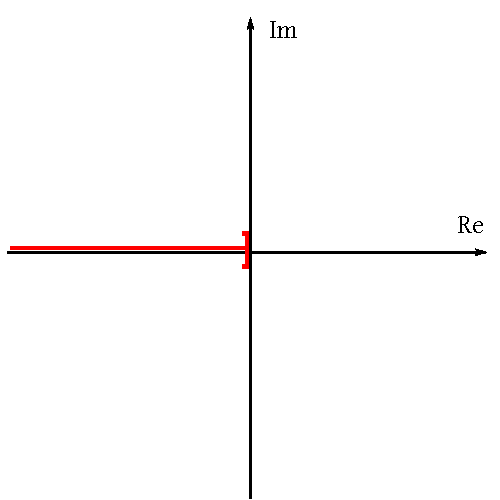
\includegraphics{img/continuous-exp-in-C.pdf}
    \caption{Continuous exponential function in $\mathbb C$}
  \end{center}
\end{figure}

\meta{lecture}{3rd of March 2016}{Wolfgang Ring}

\subsection{Further remarks on differential calculus}

\begin{theorem}
  Let $f: I \to \mathbb R$ be strictly monotonically increasing (or s. m. decreasing)
  where $I$ is an interval. Then $f^{-1}: f(I) \to \mathbb R$ is defined and the inverse function.

  Let $f$ in $x_0 \in I$ be differentiable and $f'(x_0) \neq 0$. Then $f^{-1}$ is in $y_0 = f(x_0)$
  differentiable and it holds that
  \[ (f^{-1})'(y_0) = \frac{1}{f'(x_0)} = \frac{1}{f'(f^{-1}(y_0))} \]
\end{theorem}

\begin{proof}
  Let $y_n \to y_0$ and $y_n \in f(I)$; $y_0 = f(x_0)$; $y_0 \in f(I)$; $y_n = f(x_n)$.
  $y_n \neq y_0 \Rightarrow x_n \neq x_0$.
  \[ \lim_{n\to\infty} \frac{f^{-1}(y_n) - f^{-1}(y_0)}{y_n - y_0} \]
  \[
    = \lim_{n\to\infty} \frac{x_n - x_0}{f(x_n) - f(x_0)}
    = \frac{1}{\lim_{n\to\infty} \underbrace{\frac{f(x_n) - f(x_0)}{x_n - x_0}}}_{\text{ex} = f'(x_0)} = \frac{1}{f'(x_0)}
  \]
\end{proof}

\begin{lemma}
  \label{lemma:const-diff}
  Let $f: I \to \mathbb R$ where $I$ is some interval. Then it holds that
  \[ f = \text{ const} \Leftrightarrow f \text{ is differentiable in $I$ and } f'(x) = 0 \forall x \in I \]
\end{lemma}
\begin{proof}
  \begin{description}
    \item[$\Rightarrow$]
      Immediate.
    \item[$\Leftarrow$]
      Let $f$ be differentiable and $f' \equiv 0$.
      Assume $f$ is not constant. Then there exist $x_1, x_2 \in I$, $x_1 \neq x_2$
      and $f(x_1) \neq f(x_2)$. Without loss of generality, $x_1 < x_2$.
      The Intermediate Value Theorem states that
      \[ \exists \xi \in (x_1, x_2) \subseteq I: f'(\xi) = \frac{f(x_2) - f(x_1)}{x_2 - x_1} \neq 0 \]
      This is a contradiction to the assumption that $f' \equiv 0$.
  \end{description}
\end{proof}

\index[English]{Primitive}
\index[German]{\foreignlanguage{ngerman}{Stammfunktion}}
\begin{defi}
  Let $I$ be an interval, $f: I \to \mathbb R$.
  A function $F: I \to \mathbb R$ is called \emph{primitive} or \emph{antiderivative} of $f$
  if $F$ is differentiable and
  \[ \forall x \in I: F'(x) = f(x) \]
\end{defi}
\begin{lemma}
  Let $f: I \to \mathbb R$. Let $F_1$ and $F_2$ be two primitive functions of $f$.
  Then it holds that $F_1 - F_2 = \text{const}$.
\end{lemma}
\begin{proof}
  $F_1$, $F_2$ are differentiable.
  \[ (F_1 - F_2)'(x) = F_1'(x) - F_2'(x) = f(x) - f(x) = 0 \]
  \[ \xRightarrow{\text{Lemma~\ref{lemma:const-diff}}} F_1 - F_2 = \text{ const} \]
\end{proof}

\begin{theorem}
  Let $I$ be an interval.
  Let $(f_n)_{n\in\mathbb N}$ be a sequence of differentiable functions in $I$.
  \[ f_n: I \to \mathbb R \text{ differentiable} \]
  Furthermore let $f: I \to \mathbb R$.
  It holds that,
  \begin{enumerate}
    \item
      $\forall x \in I$ let $f(x) = \lim_{n\to\infty} f_n(x)$
      ($f_n \to f$ pointwise)
    \item
      for every $x \in I$ let $(f'_n(x))_{n\in\mathbb N}$ be convergent
      (hence $\varphi(x) = \lim_{n\to\infty} f_n'(x)$ exists for every $x$)
    \item
      $\forall \varepsilon > 0 \exists N \in \mathbb N$ such that
      \[ n \geq N \Rightarrow \abs{(f_n - f)(u) - (f_n - f)(v)} \leq \varepsilon \abs{u - v} \forall u,v \in I \]
      Then $f$ is differentiable in $I$ and it holds that $f'(x) = \varphi(x) = \lim_{n\to\infty} f'_n(x)$.
      \[ f'(x) = [\lim_{n\to\infty} f]'(x) \]
  \end{enumerate}
\end{theorem}
\begin{proof}
  Let $x_0 \in I$ and $x \in I$. Let $\varepsilon > 0$ arbitrary.
  \[ \abs{\frac{f(x) - f(x_0)}{x - x_0} - \varphi(x_0)} \]
  \[ = \abs{\frac{f(x) - f(x_0)}{x - x_0} - \lim_{n\to\infty} f_N'(x_0)} \]
  \[ = \abs{\frac{f(x) - f(x_0)}{x - x_0} - f'_N(x_0)} + \abs{f'_N(x_0) - \lim_{n\to\infty} f'_n(x_0)} \forall N \in \mathbb N \]
  \[
    \leq \abs{\frac{f(x) - f(x_0)}{x - x_0} - \frac{f_N(x) - f_N(x_0)}{x - x_0}}
  \] \[
    + \abs{\frac{f_N(x) - f_N(x_0)}{x - x_0} - f'_N(x_0)}
    + \abs{f'_N(x_0) - \varphi(x_0)}
  \]

  \begin{description}
    \item[1st term]
      \[
        \abs{\frac{(f(x) - f_N(x)) - (f(x_0) - f_N(x_0))}{x - x_0}}
        = \abs{\frac{(f - f_N)(x) - (f - f_N)(x_0)}{x - x_0}}
      \] \[
        \leq \frac\varepsilon3 \frac{\abs{x - x_0}}{\abs{x - x_0}}
        \stackrel{\text{condition 3}}{=} \frac{\varepsilon}{3}
      \]
      for sufficiently large $N$.
    \item[3rd term]
      $\abs{f'_N(x_0) - \varphi(x)} < \frac{\varepsilon}{3}$ for sufficiently large $N$.
  \end{description}

  Now let $N$ be fixed (with a value such that the first and third term is less than $\frac\varepsilon3$).

  \begin{description}
    \item[2nd term]
      \[ \abs{\frac{f_N(x) - f_N(x_0)}{x - x_0}} - f'_N(x_0) \]
  \end{description}

  Differentiability of $f_N$:
  Therefore for $\abs{x - x_0} < \delta$.
  \[
    \abs{\frac{f(x) - f(x_0)}{x - x_0} - \varphi(x_0)}
    < \frac\varepsilon3 + \frac\varepsilon3 + \frac\varepsilon3
    = \varepsilon
  \]
  $f$ is differentiable in $x_0$ and $f'(x_0) = \varphi(x_0)$.
\end{proof}

\begin{theorem}
  Let $f_n: I \to \mathbb R$ and $f: I \to \mathbb R$ ($n \in \mathbb N$)
  and $f_n$ is differentiable in $I$.

  Assumption:
  \begin{enumerate}
    \item $f_n \to f$ converges pointwise in $I$
      (like the first statement in the previous Theorem)
    \item There exists $g: I \to \mathbb R$ such that
      $f'_n \to g$ is continuous in $I$
  \end{enumerate}
  Then $f$ is differentiable in $I$ and it holds that
  \[ f'(x_0) = g(x_0) \quad \forall x_0 \in I \]
\end{theorem}

\meta{lecture}{4th of March 2016}{Wolfgang Ring}

\begin{theorem}[Reminder of theorem]
  \label{thm:diff-conv}
  Let $(f_n)_{n\in\mathbb N}$ be a sequence of functions in $I$ and
  let $f_n$ be differentiable $\forall n \in \mathbb N$. Furthermore,
  \begin{itemize}
    \item $f_n \to f$ pointwise
    \item $f'_n(x) \to \varphi(x)$ for every $x$
    \item $\forall \varepsilon > 0 \forall u,v \in I \exists N: n \geq N
      \Rightarrow \abs{(f_n - f)(u) - (f_n - f)(v)} < \varepsilon \abs{u - v}$
  \end{itemize}
  Then it holds that $f$ is differentiable and $f'(x) = \varphi(x) \forall x \in I$.
\end{theorem}

Conclusion:
\begin{theorem}
  \label{thm:concl}
  Let $f_n$ and $f$ be differentiable as in Theorem~\ref{thm:diff-conv}:
  $f_n: I \to \mathbb R$ and $f: I \to \mathbb R$ and it holds that
  \begin{itemize}
    \item $f_n \to f$ pointwise in $I$ for $n \to \infty$
    \item $\exists g: I  \to \mathbb R$ such that $f'_n \to g$ is \emph{uniform} in $I$,
      hence $\forall \varepsilon > 0 \exists N \in \mathbb N:
      n \geq N \land x \in I \Rightarrow \abs{f'_n(x) - g(x)} < \varepsilon$
  \end{itemize}
  Then $f$ is differentiable in $I$ and $f'(x) = g(x) \forall x \in I$.
\end{theorem}
\begin{proof}
  We check whether the two conditions lead to the conditions of Theorem~\ref{thm:diff-conv}.

  We look at the conditions of Theorem~\ref{thm:diff-conv}:
  \begin{itemize}
    \item[2.] Uniform convergences of $f'_n \to g$ implies pointwise convergence
      \[ \forall x \in I: f'_n(x) \to g(x) \]
    \item[3.] From uniform convergence of $f'_n \to g$ it follows that
      Let $\varepsilon > 0$ be arbitrary and $N$ is sufficiently large enough, such that
      $\forall n \geq N$ and $\forall x \in I$:
      \[ \abs{f_n'(x) - g(x)} < \frac\varepsilon2 \]
      Choose $n,m \geq N$ and $x \in I$ arbitrary. Then it holds that
      \[ \abs{f'_n(x) - f'_m(x)} = \abs{f'_n(x) - g(x) + g(x) - f'_m(x)} \]
      \[ \leq \abs{f'_n(x) - g(x)} + \abs{g(x) - f'_m(x)} < \frac\varepsilon2 + \frac\varepsilon2 = \varepsilon \]
      So $(f_n)_{n\in\mathbb N}$ is a uniform Cauchy sequence.

      Let $\varepsilon > 0$ be arbitrary and $N$ such that $n,m \geq N$ and $x \in I$:
      \[ \abs{f'_n(x) - f'_m(x)} < \varepsilon \]

      Consider the third condition of Theorem~\ref{thm:diff-conv}. Let $u,v \in I$
      \[ \abs{(f - f_n)(u) - (f - f_n)(v)} = \lim_{m\to\infty} \abs{(f_m - f_n)(u) - (f_m - f_n)(v)} \]
      where $(f_m - f_n)$ and $(f_m - f_n)$ is differentiable. Then according to the
      mean value theorem of differential calculus (dt. Mittelwertsatz der Differentialrechnung)
      \begin{align*}
        &= \lim_{m\to\infty} \abs{(f_m - f_n)'(\xi_{m,n}) \cdot (u - v)} \\
        &= \lim_{m\to\infty} \abs{f'_m(\xi_{m,n}) - f'_n(\xi_{m,n})} \cdot \abs{u - v}
      \end{align*}
      For $m \geq N$:
      \[ \leq \varepsilon \cdot \abs{u - v} \]
      So the third condition of Theorem~\ref{thm:diff-conv} is satisfied.
  \end{itemize}
\end{proof}

\begin{figure}[!h]
  \begin{center}
    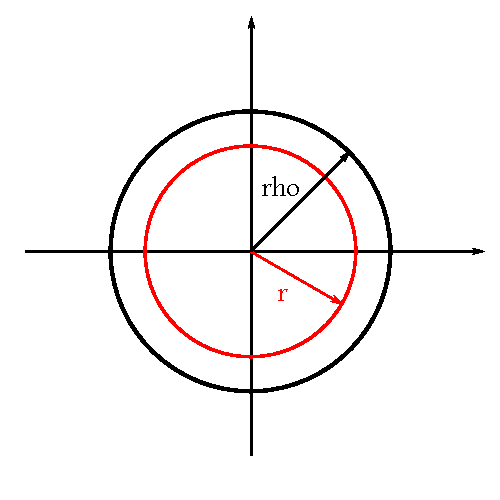
\includegraphics{img/convergence_radius.pdf}
    \caption{Convergence radius}
    \label{fig:convr}
  \end{center}
\end{figure}


\begin{rem}[An application of Theorem~\ref{thm:concl}]
  Let $P(z) = \sum_{k=0}^\infty a_k z^k$ be a power series with convergence radius $\rho(P)$ with
  \[ \rho(P) = \frac1L \qquad L = \limsup_{n\to\infty} \sqrt[n]{\abs{a_n}} \]
  \[ P_n(z) = \sum_{k=0}^n a_k z^k \qquad \text{\dots $n$-th partial sum} \]
  Let $r < \rho(P)$. Then it holds that $P_n(z) \to P(z)$ uniform in $\overline{B(0,r)}$~\footnote{Where overline means \enquote{closed}}.
  \[ P_n(x) \to P(x) \forall x \in [-r, r] \]

  Compare with Figure~\ref{fig:convr}.

  \[ P'_n(x) = \sum_{k=0}^n a_k k \cdot x^{k-1} = \sum_{j=0}^{n-1} a_{j+1} (j + 1) x^j \]
  is the $n-1$-th partial sum.
  \[ Q(z) = \sum_{j=0}^\infty a_{j+1} (j + 1) z^j \]
  Convergence radius of $Q$?
  \[ \tilde{L} = \limsup_{j\to\infty} \sqrt[j]{a_{j+1}} \cdot \sqrt[j]{j + 1} = \limsup_{j \to \infty} \abs{a_{j+1}}^{\frac{j+1}{j} \cdot \frac{1}{j+1}} \cdot (j+1)^{\frac{j+1}{j} \cdot \frac{1}{j+1}} \]
  \[
    = \limsup_{j\to\infty} \underbrace{\left(\abs{a_{j+1}}^{\overbrace{\frac{1}{j+1}}^{\to 1}}\right)^{\frac{j+1}{j}}}_{L^1 = L}
    \cdot \underbrace{\lim_{j\to\infty} \left[(j+1)^{\frac{1}{j+1}}\right]^{\frac{j+1}{j}}}_{1^1}
    = L
  \]
  In conclusion we have $\tilde L = L$ and $\rho(Q) = \frac1{L} = \rho(P)$.
  So $P'_n(z) = \sum_{k=1}^n k \cdot a_k z^{k-1}$ uniformly convergent in $\overline{B(0,r)}$ for $r<\rho$
  and therefore also uniformly convergent  in $[-r,r]$.

  From Theorem~\ref{thm:diff-conv} (or \ref{thm:concl}?) it follows that $P(x)$ is differentiable % TODO: or?
  in $[-r,r]$ and $P'(x) = \sum_{k=1}^\infty k \cdot a_k \cdot x^{k-1}$.

  Let $\abs{x} < \rho(P)$. Let $r = \frac12 (\abs{x} + \rho(P))$, then it holds that
  $x \in [-r, r]$ and $P$ is differentiable in point $x$ with
  \[ P'(x) = \sum_{k=1}^\infty k \cdot a_k \cdot x^{k-1} \]
\end{rem}

\begin{lemma}
  Let $P(z) = \sum_{k=0}^\infty a_k z^k$ be a power series with convergence radius $\rho(P) > 0$.
  Let $x \in (-\rho(P), \rho(P))$. Then $P$ is differentiable in $x$ and it holds that
  \[ P'(x) = \sum_{k=1}^\infty k \cdot a_k \cdot x^{k-1} \]

  Furthermore the power series $\sum_{k=1}^\infty k \cdot a_k \cdot x^{k-1}$ is uniformly convergent
  in every interval $[-r, r]$ with $0 < r < \rho(P)$.
\end{lemma}

\subsection{About logarithm functions}
%
We consider the power series
\[ g(z) = \sum_{k=1}^\infty \frac{z^k}{k} \]
\[ \rho(g) = \frac1L \text{ with } L = \limsup_{k\to\infty} \sqrt[k]{\frac1k} = \frac{1}{\lim_{k\to\infty} \sqrt[k]{k}} = 1 \]
So it holds that $\rho(g) = 1$.

Apply the previous theorem, followingly $g$ is differentiable in $(-1,1)$ and it holds that
\[ g'(x) = \sum_{k=1}^\infty \frac{k}{k} x^{k-1} = \sum_{j=0}^\infty x^j = \frac1{1 - x} \]

Remark:
\[ \left[-\ln(1 - x)\right]' = -\frac{1}{1 - x} \cdot (-1) = \frac1{1 - x} \]
\[ \Rightarrow \sum_{k=1}^\infty \frac{x^k}{k} + \ln(1 - x) = \text{ constant} \]
Let $x = 0$ (we determine the constant for this $x=0$):
\[ 0 + 0 = 0 = \text{ constant} \]
\[ \Rightarrow \ln(1 - x) = -\sum_{k=1}^\infty \frac{x^k}{k} \qquad \text{ for } \abs{x} < 1 \]

Let $x \in (-1,1) \Rightarrow -x \in (-1,1)$.
\[ \Rightarrow \ln(1 - (-x)) = \ln(1 + x) = -\sum_{k=1}^\infty \frac{(-x)^k}{k} \]
\[ = \sum_{k=1}^\infty \frac{(-1)^{k-1} \cdot x^k}{k} = x - \frac{x^2}{2} + \frac{x^3}{3} - \frac{x^4}{4} + \ldots \]

\index[English]{Logarithmic series}
\index[German]{\foreignlanguage{ngerman}{Logarithmische Reihe}}
Therefore: We introduce \emph{logarithmic series}:
\[ \ln(1 - x) = -\sum_{k=1}^\infty \frac{x^k}{k} \]
\[ \ln(1 + x) = \sum_{k=1}^\infty \frac{(-1)^{k-1} x^k}{k} \]
\[
  \ln\left(\frac{1 + x}{1 - x}\right)
  = \ln(1 + x) - \ln(1 - x)
  = 2 \sum_{l=1}^\infty \frac{x^{2l - 1}}{2l - 1}
  \quad \text{ for } x \in (-1,1)
\]

\begin{figure}[!h]
  \begin{center}
    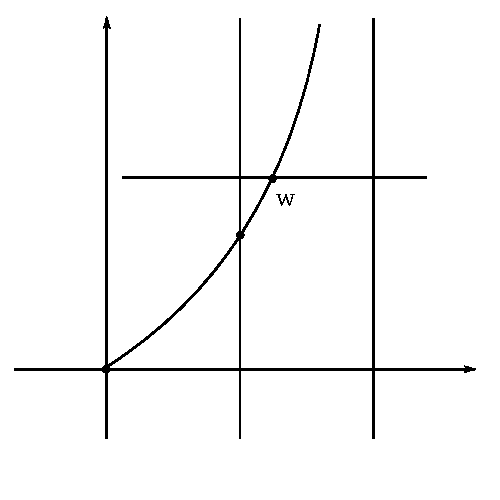
\includegraphics{img/1x_1-x.pdf}
    \caption{Plot of $\frac{1+x}{1-x}$}
    \label{img:1x-1x}
  \end{center}
\end{figure}

\[ f(x) = \frac{1 + x}{1 - x} \]
Compare with Figure~\ref{img:1x-1x}.
\[ f'(x) = \frac{1 - (-1)}{(1 - x)^2} = \frac{2}{(1 - x)^2} > 0 \quad \text{ in } (-1, 1) \]
Solve $\frac{1 + x}{1 - x} = w$ for $x$.

\[ \Rightarrow 1 + x  = w - wx \]
\[ x (1 + w) = w - 1 \]
\[ x = \frac{w - 1}{w + 1} \]

\[ \ln(w) = 2 \sum_{l=1}^\infty \frac{x^{2l-1}}{2l - 1} \]

\section{Trigonometic functions}

We define trigonometic functions using the exponential function in $\mathbb C$.

Let $t \in \mathbb R$.
\[ e^{it} = \sum_{k=0}^\infty \frac{(it)^k}{k!} = \lim_{n\to\infty} \left(\underbrace{1}_{\mathbb R} + \underbrace{\frac{it}{n}}_{i \mathbb R}\right)^n \]
\[
  e^{-it}
    = \lim_{n\to\infty} \left(1 - \frac{it}{n}\right)^n
    = \lim_{n\to\infty} \left[\overline{\left(1 + \frac{it}{n}\right)}\right]^n
\] \[
  = \lim_{n\to\infty} \overline{\left(1 + \frac{it}{n}\right)^n}
  = \overline{\lim_{n\to\infty} \left(1 + \frac{it}{n}\right)^n}
  = e^{it}
\] \[
  \abs{e^{it}}^2 = e^{it} \cdot \overline{e^{it}} = e^{it} \cdot e^{-it}
\] \[
  e^{it - it} = e^0 = 1
\]
So it holds that $\forall t \in \mathbb R$:
\[ \abs{e^{it}} = 1 \]
So $e^{it}$ lies inside the complex unit circle. Compare with Figure~\ref{img:unitc}.

\begin{figure}[!h]
  \begin{center}
    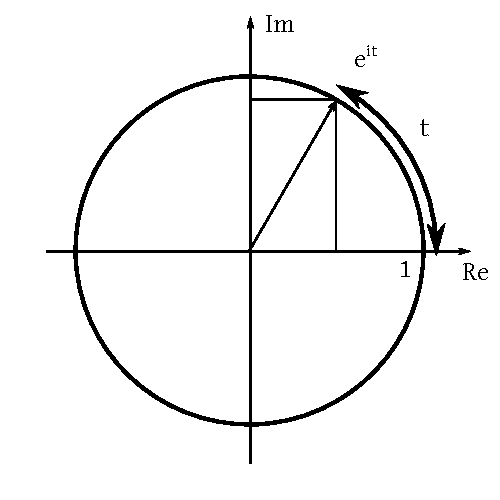
\includegraphics{img/unitcircle_in_C.pdf}
    \caption{Unit circle in $C$ with $t$}
    \label{img:unitc}
  \end{center}
\end{figure}

\index[English]{Sine function}
\index[German]{\foreignlanguage{ngerman}{Sinusfunktion}}
\index[English]{Cosine function}
\index[German]{\foreignlanguage{ngerman}{Cosinusfunktion}}
We define the cosine function $\cos: \mathbb R \to \mathbb R$ as
\[ \cos(t) = \Re(e^{it}) \]
and the sine function $\sin: \mathbb R \to \mathbb R$ as
\[ \sin(t) = \Im(e^{it}) \]

The following relations hold:
\begin{enumerate}
  \item $e^{it} = \cos(t) + i \cdot \sin(t)$ (Euler's identity)
  \item $\abs{e^{it}}^2 = 1 = (\cos{t})^2 + (\sin{t})^2$
  \item \[ \Re(z) = \frac12 (z + \overline{z}) \]
    \[ \Rightarrow \cos(t) = \Re(e^{it}) = \frac12 \left(e^{it} + e^{-it}\right) \]
    \[ \Im(z) = \frac1{2i} [z - \overline{z}] \]
    \[ \sin(t) = \Im(e^{it}) = \frac{1}{2i} \left[e^{it} - e^{-it}\right] \]
  \item
    \[ e^{-it} = \overline{e^{it}} = \cos{t} - i \cdot \sin{t} \]
\end{enumerate}

We use property 3 to extend the domain of sine and cosine:
\begin{defi}
  Let $z \in \mathbb C$. We define $\sin: \mathbb C \to \mathbb C$
  and $\cos: \mathbb C \to \mathbb C$ by
  \[ \cos(z) = \frac12 \left[e^{iz} + e^{-iz}\right] \]
  \[ \sin(z) = \frac1{2i} \left[e^{iz} - e^{-iz}\right] \]
\end{defi}


\clearpage
\begin{otherlanguage}{ngerman}
\printindex[German]
\end{otherlanguage}
\printindex[English]

\end{document}

%%% Local Variables:
%%% mode: latex
%%% TeX-master: t
%%% End:
